\section{Geografska karta penjališta}

Kako bi se korisnicima olakšala prostorna orijentacija, aplikacije integriraju interaktivnu geografsku kartu. Ova funkcionalnost omogućuje vizualno istraživanje penjališta na globalnoj razini kao i detaljnu navigaciju unutar pojedine penjališta.

\begin{figure}[H]
    \centering
    \begin{subfigure}[b]{\textwidth}
        \centering
        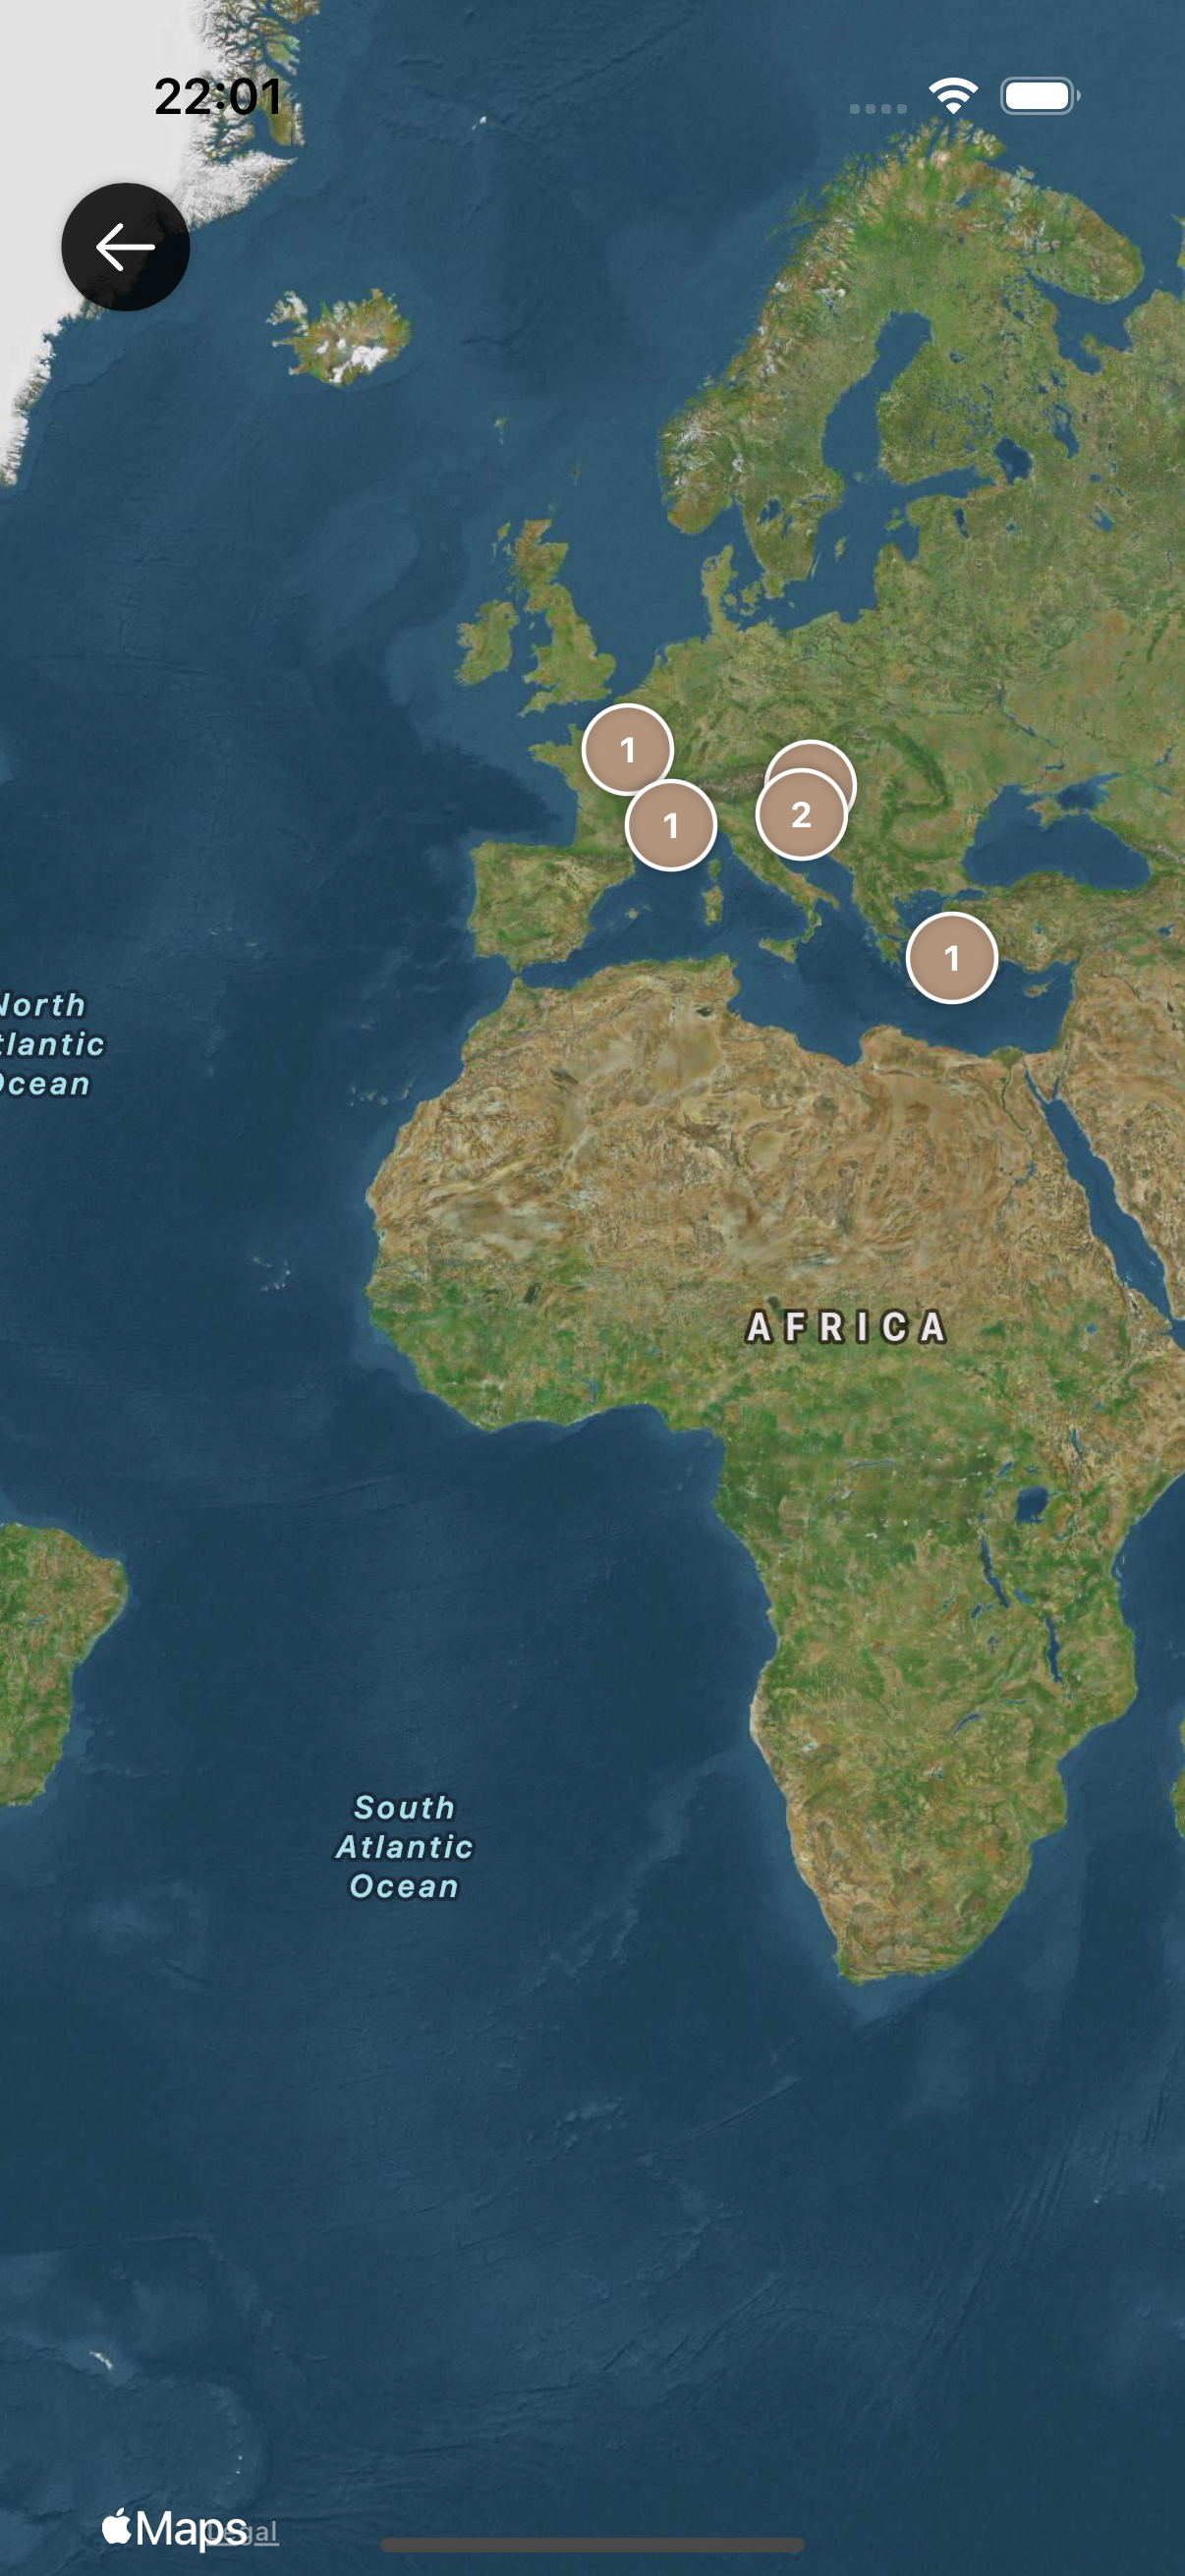
\includegraphics[width=0.3\textwidth]{images/implementacija/geo_karta.png}
        \caption{Mobilna aplikacija}
        \label{fig:geografska_karta_mob}
    \end{subfigure}
    \hfill
    \begin{subfigure}[b]{\textwidth}
        \centering
        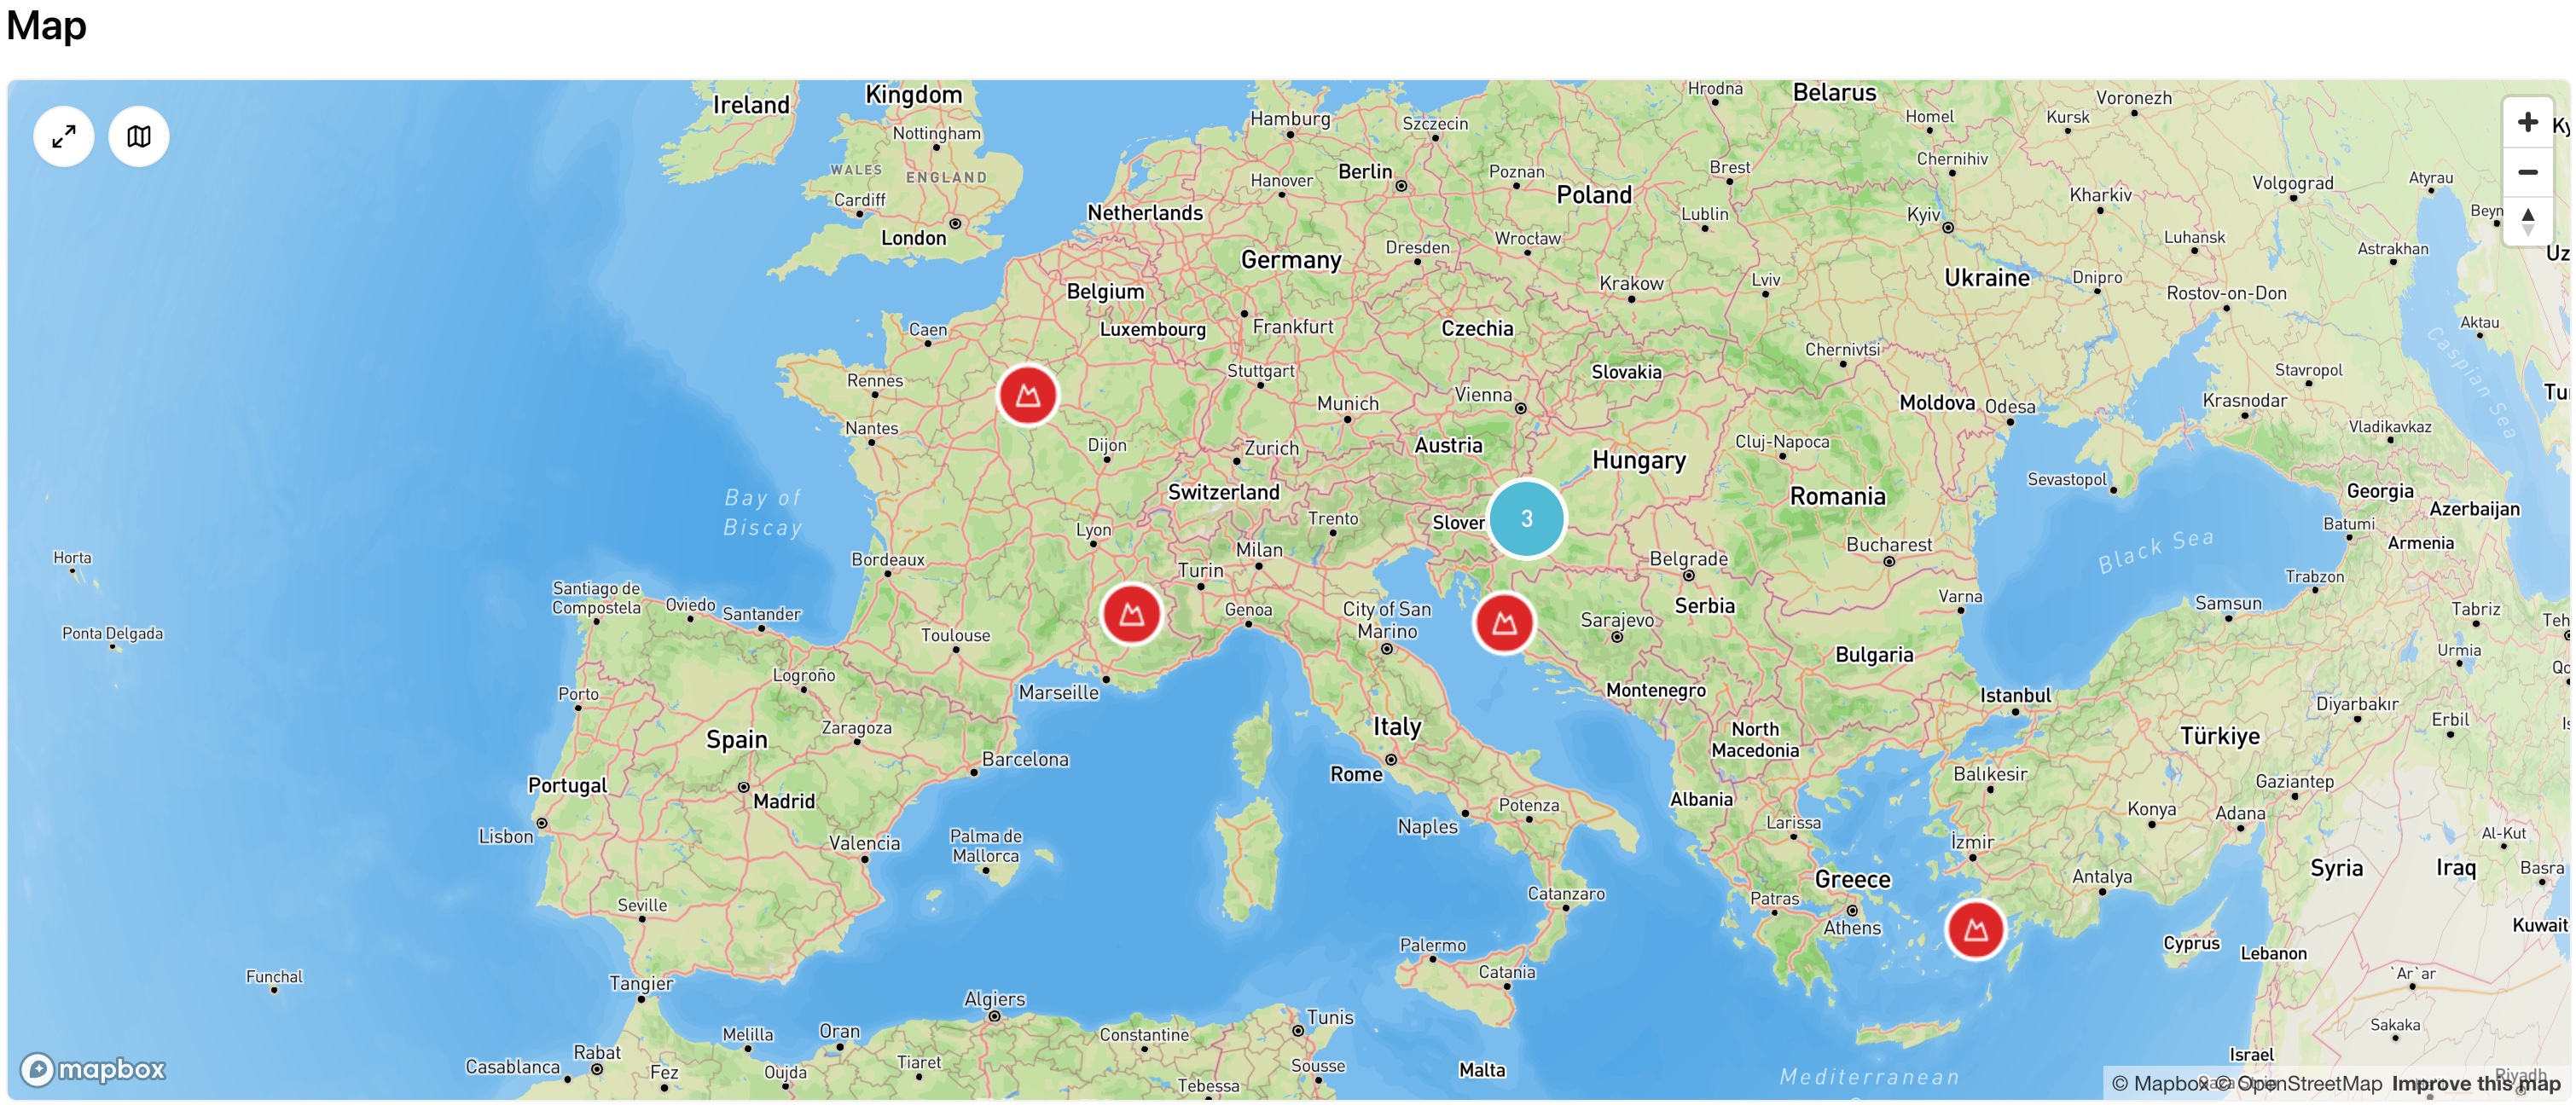
\includegraphics[width=0.9\textwidth]{images/implementacija/web/map_clusters.jpeg}
        \caption{Web aplikacija}
        \label{fig:geografska_karta_web}
    \end{subfigure}
    \caption{Geografska karta penjališta s prikazom grupiranih oznaka}
    \label{fig:geografska_karta_sidebyside}
\end{figure}

Pristupom karti korisniku se prikazuje karta svijeta (slika~\ref{fig:geografska_karta_sidebyside}) s grupiranim oznakama (eng. \textit{clusters}) koje indiciraju broj dostupnih penjališta na određenom području. Grupirane oznake omogućuju pregled penjališta na visokoj razini, ali bez pretrpanosti informacijama. Približavanjem karte, grupirane oznake se razdvajaju, otkrivajući pojedinačna penjališta.

\begin{figure}[H]
    \centering
    \begin{subfigure}[b]{\textwidth}
        \centering
        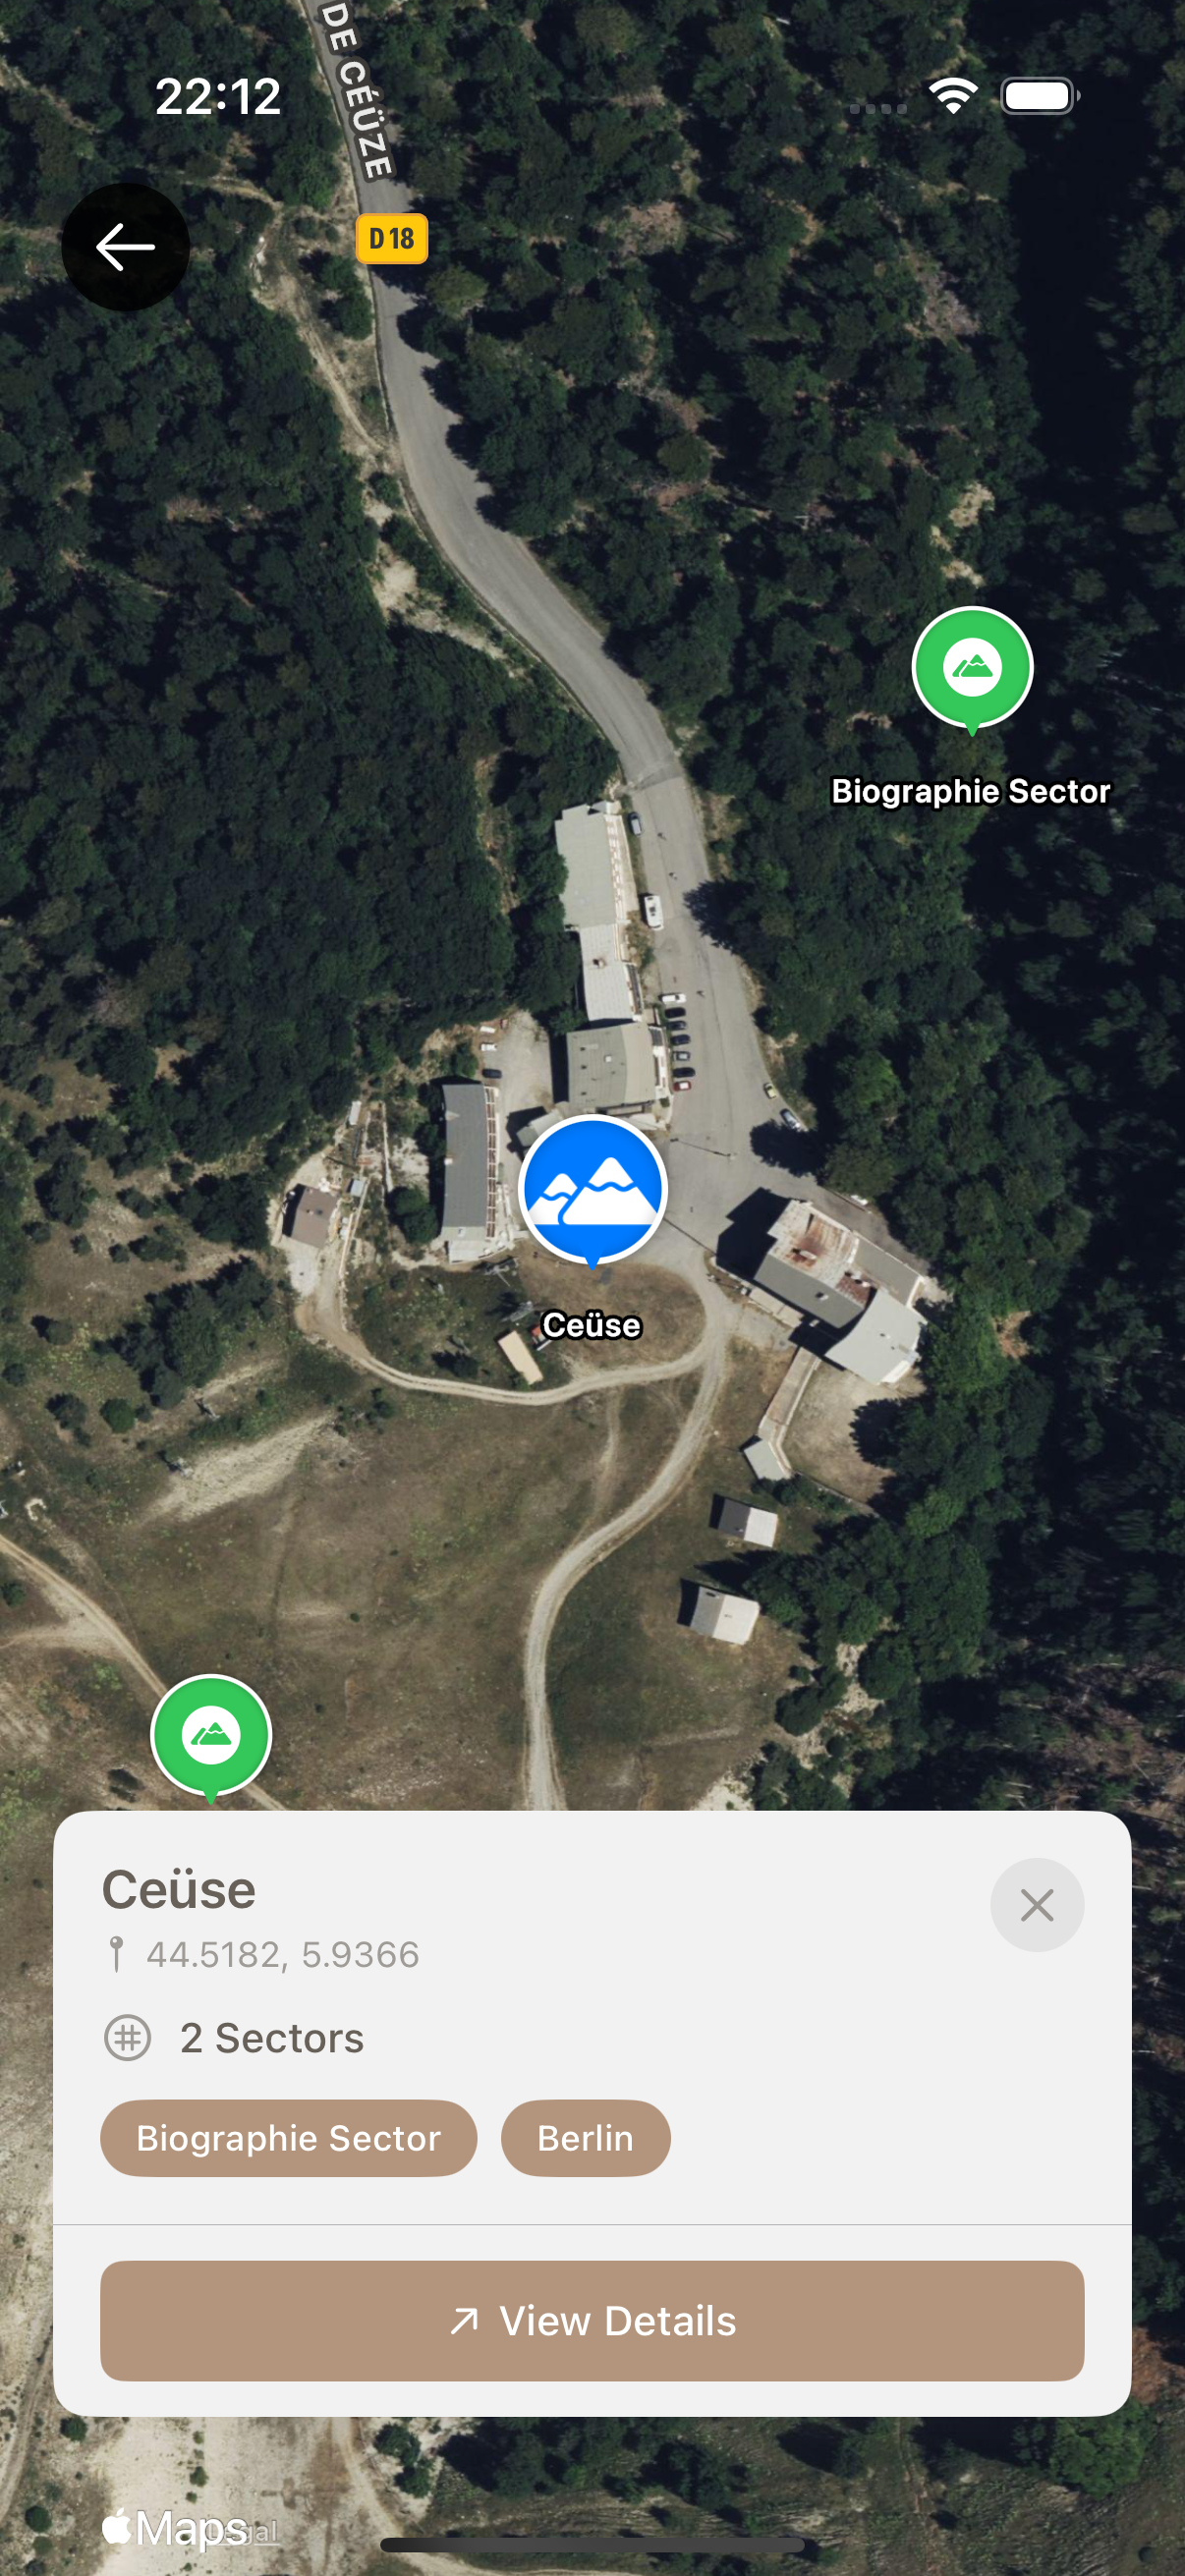
\includegraphics[width=0.3\textwidth]{images/implementacija/geo_karta_ceuse.png}
        \caption{Mobilna aplikacija}
        \label{fig:geografska_karta_ceuse_mob}
    \end{subfigure}
    \hfill
    \begin{subfigure}[b]{\textwidth}
        \centering
        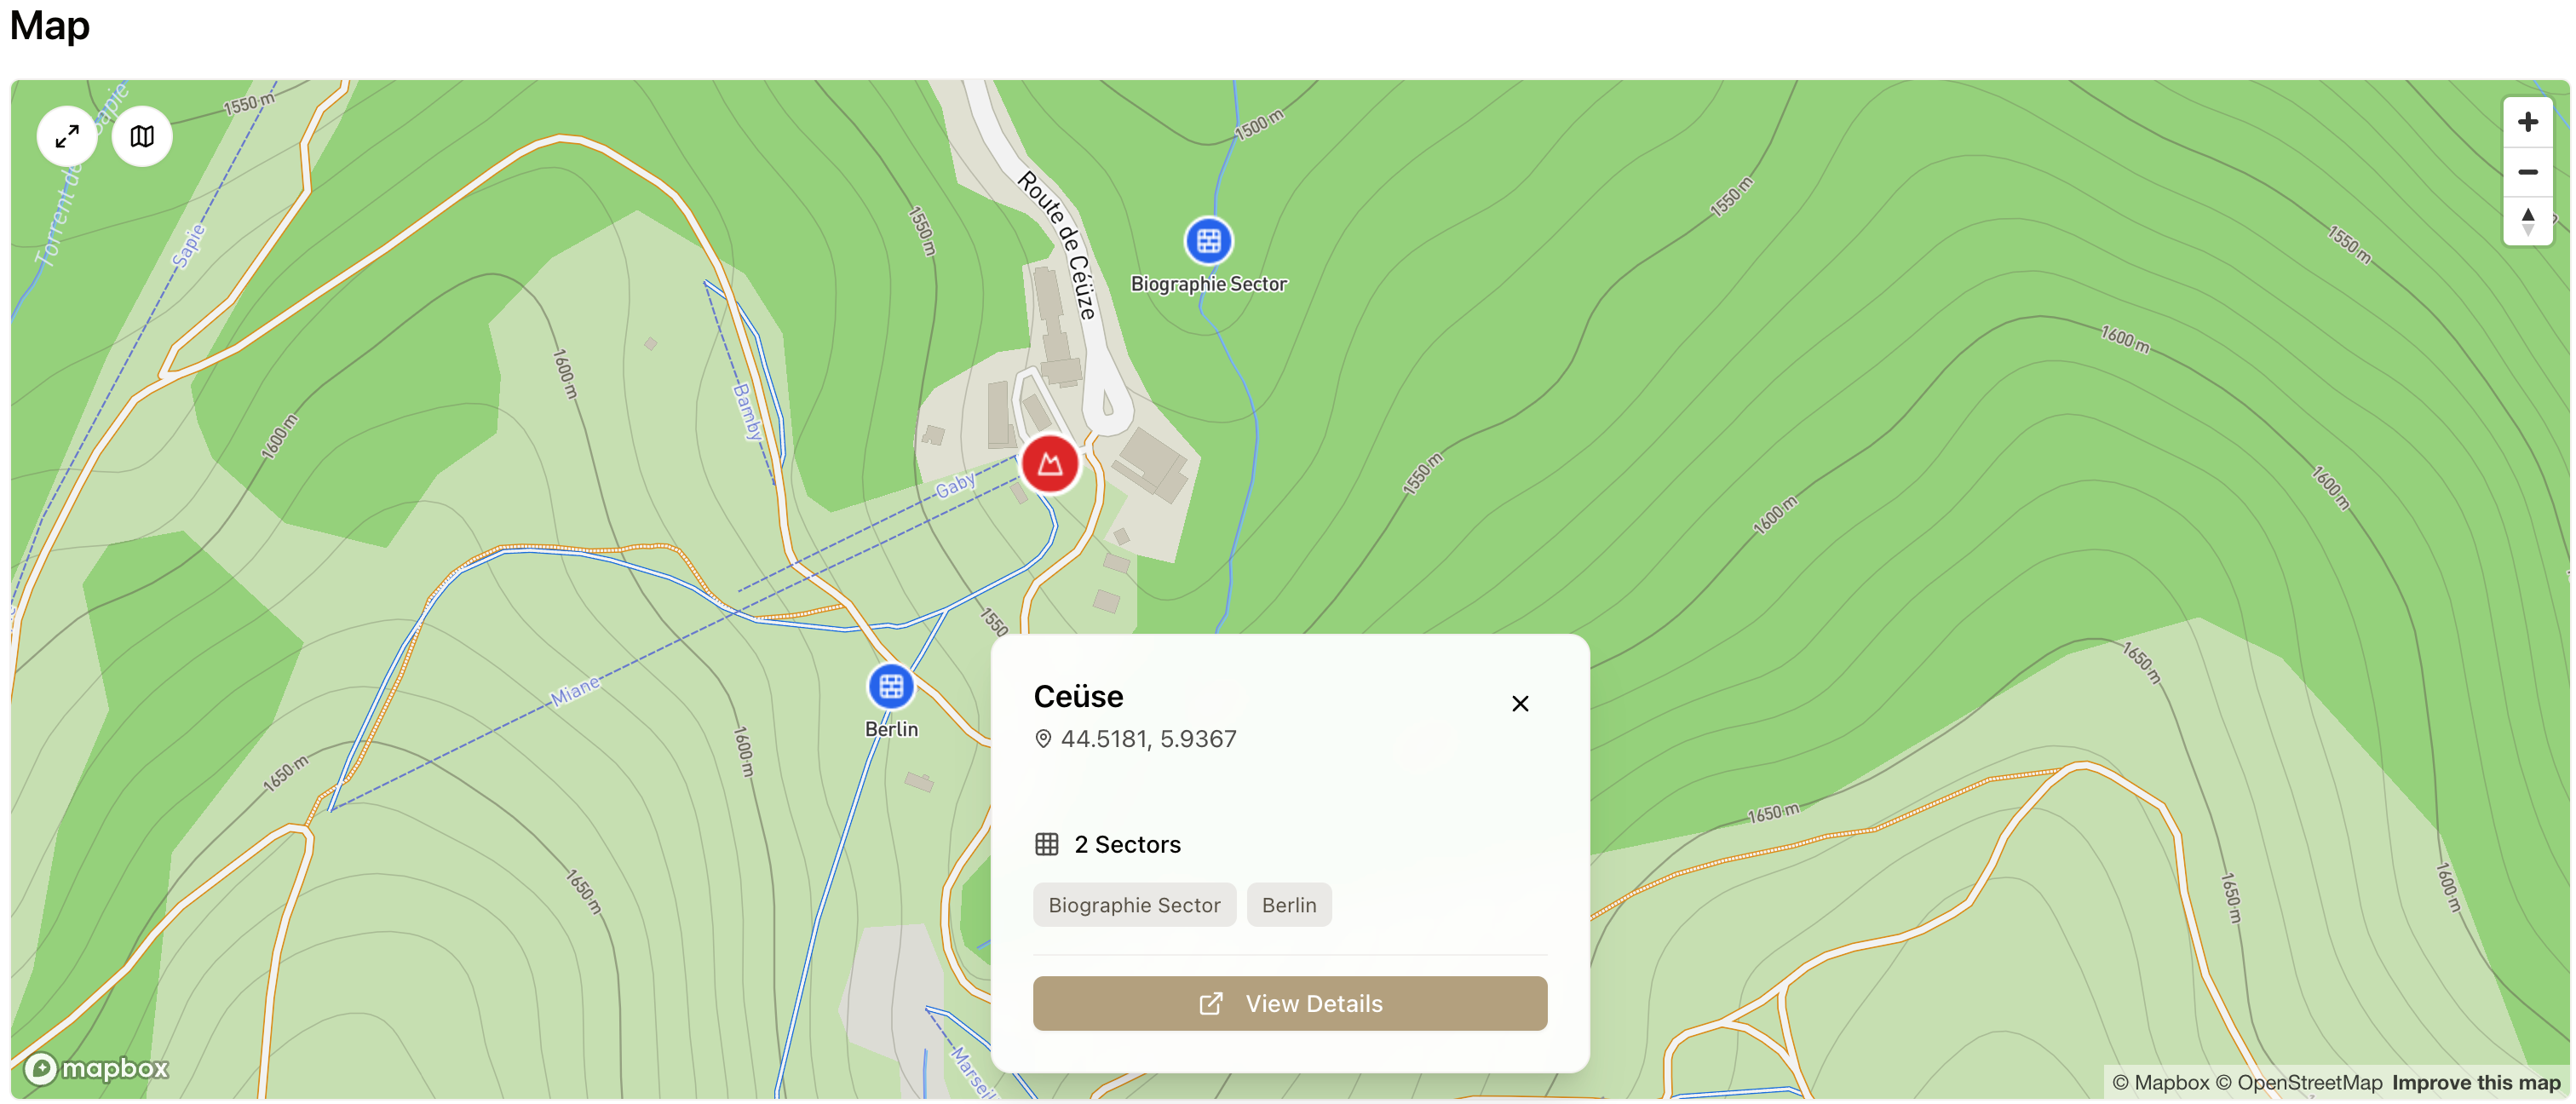
\includegraphics[width=0.9\textwidth]{images/implementacija/web/map_selected.png}
        \caption{Web aplikacija}
        \label{fig:geografska_karta_ceuse_web}
    \end{subfigure}
    \caption{Detaljan prikaz penjališta Ceuse}
    \label{fig:geografska_karta_ceuse_sidebyside}
\end{figure}

Odabirom oznake za pojedino penjalište, karta se automatski centrira i približava na tu lokaciju, prikazujući satelitski snimak područja (slika~\ref{fig:geografska_karta_ceuse_sidebyside}). Na ovom detaljnom prikazu prikazana je oznaka za penjalište, a i oznake za sve sektore. Ovakav prikaz je koristan za razumijevanje rasporeda sektora i planiranje kretanja na terenu. Na dnu prikaza nalazi se informativna kartica s osnovnim podacima o odabranoj lokaciji poput naziva, GPS koordinata i popisa dostupnih sektora. Korisniku se tada nude opcije za pregled detaljnih informacija o toj penjalištu ili sektorima klikom na "Pogledaj detalje" (eng. \textit{View Details}) ili klikom na željeni sektor.
